\documentclass[11pt]{article}
\usepackage[a4paper,margin=1in]{geometry}
\usepackage{graphicx}
\usepackage{booktabs}
\usepackage{amsmath}
\usepackage{hyperref}
\usepackage{tikz}
\usepackage{float}
\usepackage{array}
\usepackage{xcolor}
\title{Project 7 (Milestone 2): Intelligent Contract Risk Analysis\\\large Team DABB.ai}
\author{Birajit Saikia \and Devaansh Kathuria \and Abhey Dua \and Bhavya Jain}
\date{April 2026}

\begin{document}
\maketitle

\begin{abstract}
This report presents Milestone 2 of Project 7, which extends the Milestone 1 contract-risk baseline with a grounded legal-assistance workflow, public-host deployment settings, PDF export, and multi-contract comparison. The system keeps the classical TF-IDF + Logistic Regression classifier intact, then layers clause-level retrieval, structured explanations, and release-ready Streamlit packaging on top of it.
\end{abstract}

\section{Introduction}
Milestone 1 established a transparent machine-learning pipeline for clause classification and risk scoring. Milestone 2 keeps that behavior intact while making the project submission-ready for a public host and adding a structured assistant layer that can explain findings using a local legal guidance corpus.

The design goals for this milestone are:
\begin{itemize}
    \item preserve the classical baseline and deterministic risk mapping from Milestone 1,
    \item add grounded assistant-style reporting without introducing fragile external dependencies,
    \item make deployment straightforward on Streamlit Community Cloud, Hugging Face Spaces, or Render,
    \item keep the workflow reproducible through pinned dependencies, tests, and documented startup commands.
\end{itemize}

\section{Problem Definition and I/O Specification}
\textbf{Input:}
\begin{itemize}
    \item Contract documents in PDF or TXT format
    \item Optional labeled CSV for supervised training
\end{itemize}

\textbf{Output (per clause):}
\begin{itemize}
    \item Predicted clause type
    \item Risk severity (Low/Medium/High)
    \item Risk score (0--100)
    \item Assistant explanation, mitigation guidance, and evidence references when available
\end{itemize}

\textbf{Disclaimer:} The output is informational only and not legal advice.

\section{System Design}
\subsection{Architecture}
Figure~\ref{fig:architecture} shows the end-to-end Milestone 2 flow.

\begin{figure}[H]
\centering
\begin{tikzpicture}[node distance=0.95cm, every node/.style={draw, rounded corners, align=center, font=\small, minimum width=2.8cm, minimum height=0.9cm}]
\node (a) {Upload PDF/TXT};
\node (b) [below=of a] {Text Extraction};
\node (c) [below=of b] {Preprocess +\\Clause Segmentation};
\node (d) [below=of c] {TF-IDF Features};
\node (e) [below=of d] {Clause Classifier\\(LogReg baseline)};
\node (f) [below=of e] {Risk Mapping\\Severity + Score};
\node (g) [below=of f] {Streamlit UI};
\node (h) [below=of g] {Export CSV / JSON / PDF};

\node (k) [right=4.0cm of c, minimum width=3.4cm] {Local Legal\\Guidance Corpus};
\node (l) [below=of k, minimum width=3.4cm] {Retrieval Index};
\node (m) [below=of l, minimum width=3.4cm] {Structured\\Assistant Report};
\node (n) [below=of m, minimum width=3.4cm] {Clause Drill-down\\+ Comparison};

\draw[->] (a) -- (b);
\draw[->] (b) -- (c);
\draw[->] (c) -- (d);
\draw[->] (d) -- (e);
\draw[->] (e) -- (f);
\draw[->] (f) -- (g);
\draw[->] (g) -- (h);
\draw[->] (k) -- (l);
\draw[->] (l) -- (m);
\draw[->] (m) -- (n);
\draw[->, dashed] (n.west) -- ++(-1.2,0) |- (g.east);
\end{tikzpicture}
\caption{Milestone 2 architecture for contract-risk analysis and grounded reporting.}
\label{fig:architecture}
\end{figure}

\subsection{Methodology}
The app follows a consistent sequence:
\begin{enumerate}
    \item extract text from PDF or TXT uploads,
    \item segment the document into clause-sized units,
    \item classify each clause with a TF-IDF + Logistic Regression model,
    \item map the predicted clause type to severity and numeric risk,
    \item retrieve relevant passages from the bundled guidance corpus,
    \item compile a structured report with mitigation guidance and evidence.
\end{enumerate}

The assistant layer is intentionally local and grounded. It does not depend on external API calls during normal operation, which keeps the demo reproducible and avoids rate-limit or network failures during grading.

\subsection{Deployment Hardening}
Milestone 2 adds public-host settings and startup documentation so the repo is submission-ready:
\begin{itemize}
    \item \texttt{streamlit_app.py} is the hosted entrypoint,
    \item \texttt{.streamlit/config.toml} sets safe Streamlit defaults,
    \item \texttt{Procfile} and \texttt{render.yaml} support Render deployment,
    \item \texttt{docs/deployment.md} captures sanity checks and startup commands,
    \item configuration paths can be overridden with environment variables when needed.
\end{itemize}

\section{Results}
\subsection{Evaluation Summary}
The evaluation CLI was run on the bundled fallback path in this workspace. The main model produced a weighted precision/recall/F1 of 1.00 on the held-out split recorded in \texttt{reports/logreg\_summary\_metrics.csv}.

\begin{table}[H]
\centering
\begin{tabular}{lccc}
\toprule
Model & Precision (weighted) & Recall (weighted) & F1 (weighted) \\
\midrule
Logistic Regression & 1.00 & 1.00 & 1.00 \\
LinearSVC & 0.00 & 0.00 & 0.00 \\
Decision Tree & 0.00 & 0.00 & 0.00 \\
\bottomrule
\end{tabular}
\caption{Evaluation snapshot from the bundled fallback dataset. The comparison models are included for completeness, but the tiny demo split is not a robust benchmarking corpus.}
\label{tab:comparison}
\end{table}

\subsection{Confusion Matrix}
Figure~\ref{fig:cm} shows the generated confusion matrix artifact saved by the evaluation CLI.

\begin{figure}[H]
\centering
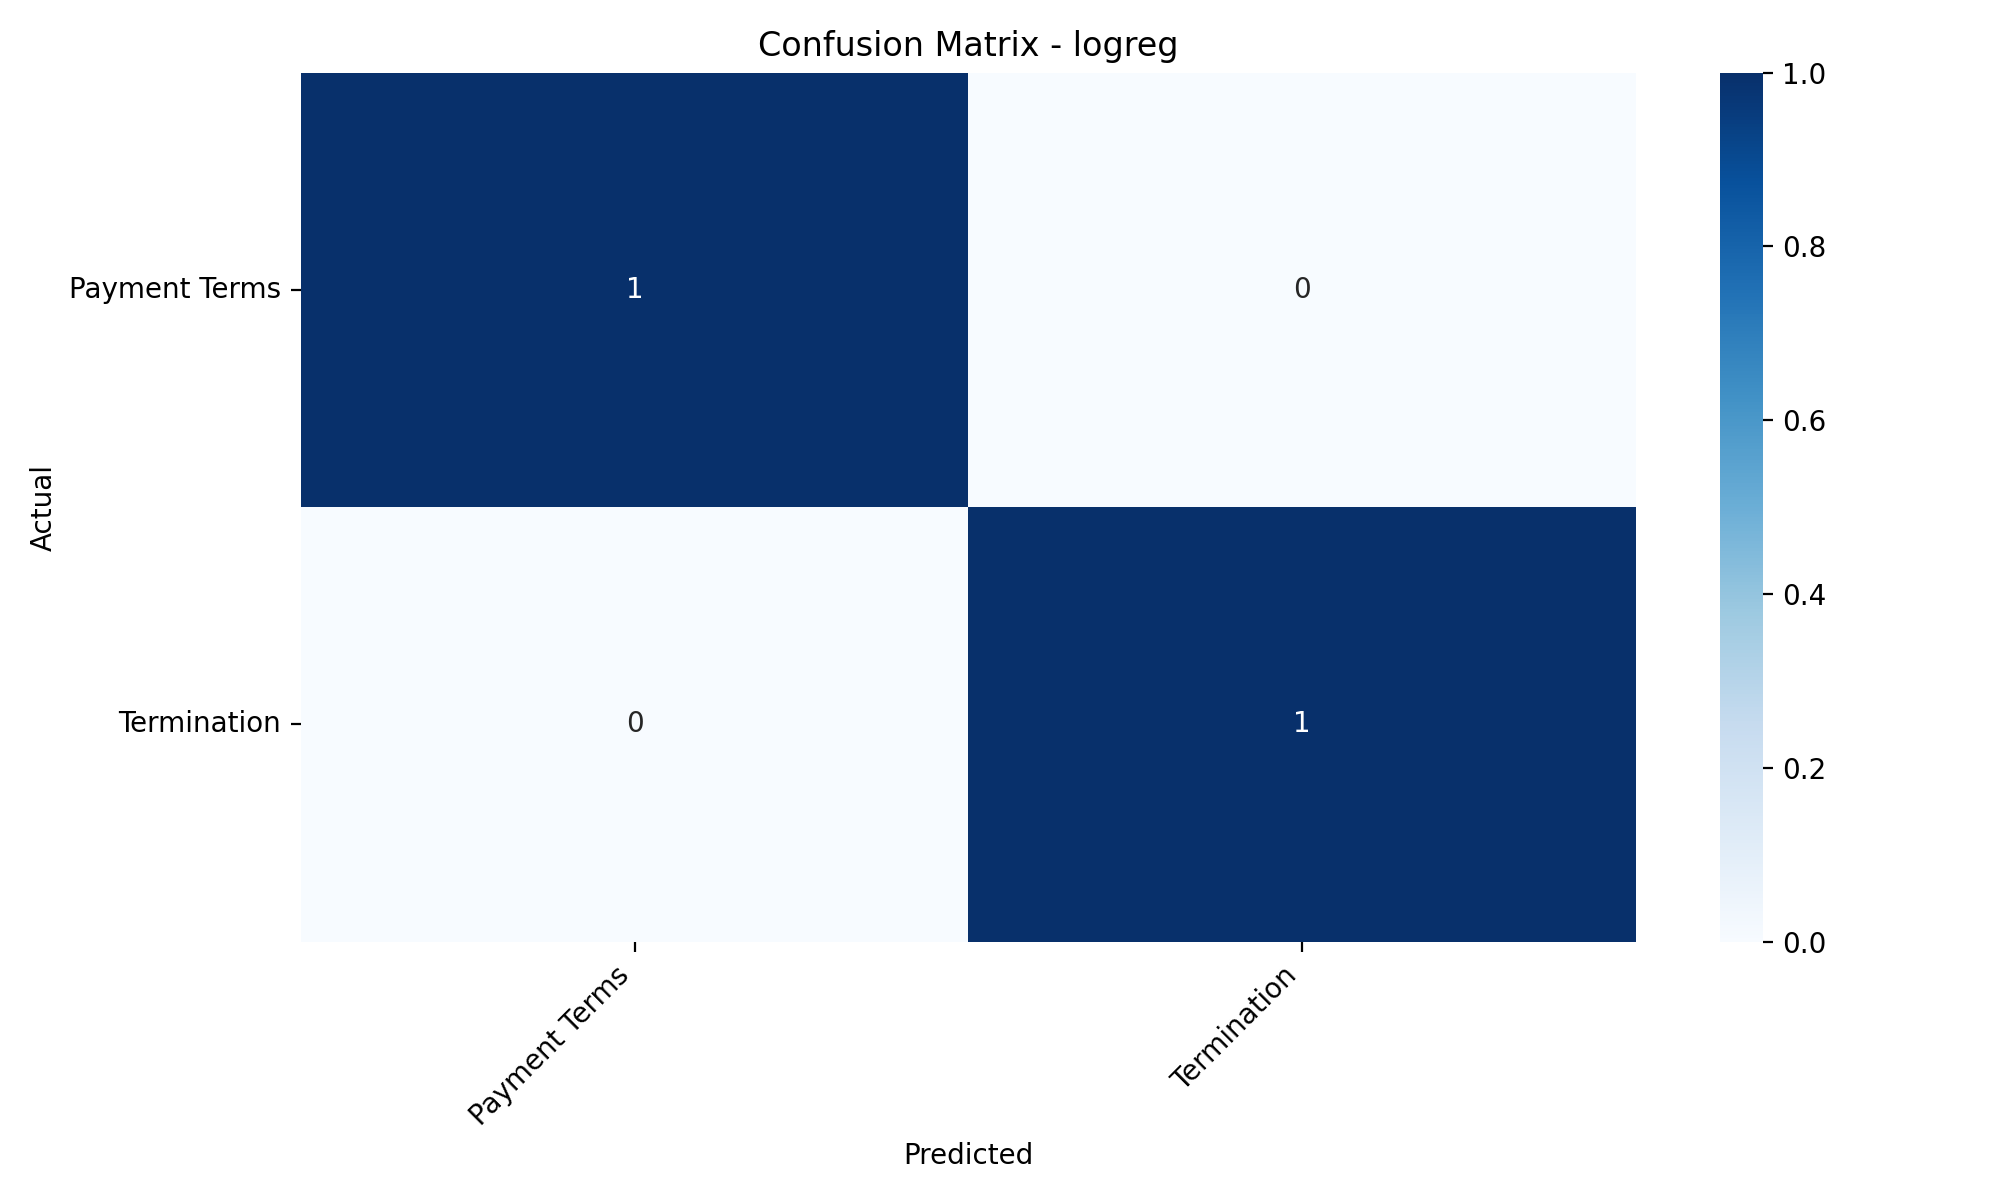
\includegraphics[width=0.9\linewidth]{figures/logreg_confusion_matrix.png}
\caption{Confusion matrix for the logistic regression baseline.}
\label{fig:cm}
\end{figure}

\subsection{Risk Mapping}
The deterministic risk table remains the core release rule:
\begin{itemize}
    \item high-severity classes include liability, indemnity, and termination patterns,
    \item medium-severity classes include arbitration, payment, and dispute-resolution clauses,
    \item low-severity classes include confidentiality and administrative wording.
\end{itemize}

\section{Application Workflow}
The Streamlit interface supports the following sequence:
\begin{itemize}
    \item upload a PDF or TXT contract,
    \item review the filtered clause table,
    \item inspect the assistant-backed report,
    \item drill into an individual clause for evidence and mitigation guidance,
    \item export CSV, JSON, or PDF outputs,
    \item compare multiple contracts for repeated risk patterns.
\end{itemize}

\section{Screenshots}
The final submission should include three app screenshots captured from the hosted deployment:
\begin{itemize}
    \item contract upload and clause analysis view,
    \item generated assistant report with evidence and mitigation guidance,
    \item multi-contract comparison view.
\end{itemize}

\begin{figure}[H]
\centering
\fbox{\parbox[c][4.2cm][c]{0.86\linewidth}{\centering
Insert the hosted app screenshot for upload + clause analysis here.}}
\caption{Submission screenshot placeholder for the main analysis screen.}
\label{fig:screenshot-main}
\end{figure}

\begin{figure}[H]
\centering
\fbox{\parbox[c][4.2cm][c]{0.86\linewidth}{\centering
Insert the hosted app screenshot for the generated report here.}}
\caption{Submission screenshot placeholder for the assistant report screen.}
\label{fig:screenshot-report}
\end{figure}

\section{Limitations}
\begin{itemize}
    \item Extracted text from scanned PDFs may still be incomplete.
    \item The fallback comparison corpus is intentionally tiny, so model-comparison metrics are illustrative rather than definitive.
    \item Risk scores are rule-based and should be treated as screening guidance.
    \item The assistant report is grounded in the bundled corpus, but it remains informational only and not legal advice.
\end{itemize}

\section{Conclusion}
Milestone 2 preserves the original classical NLP pipeline while adding a grounded report layer, deployment-safe startup settings, and presentation-ready release material. The result is a reproducible submission that can be run locally or hosted publicly with minimal setup.

\bibliographystyle{plain}
\bibliography{references}

\end{document}
